\chapter{Estudo de caso (QIE)}
Neste capítulo será descrita a utilização do processo de alinhamento através de um estudo de caso, o QIE. O QIE foi escolhido, pois se trata de um projeto que pretende cruzar informações sobre a comunidade brasileira de informática na educação.

Para validar a eficácia da solução, foi solicitado a membros da comunidade que sugerissem perguntas de seu interesse. Como resultado foi levantado um conjunto contendo mais de 30 questões (ver Tabela \ref{tab:questions}).

\begin{table}[!ht]
\centering
\caption{Perguntas sugeridas pela comunidade}
\label{tab:questions}
\begin{tabular}{|l|l|}
\hline
ID  & Questões                                                                          \\ \hline
Q01 & Quantos pesquisadores?                                                            \\ \hline
Q02 & Quais pesquisadores?                                                              \\ \hline
Q03 & Onde estão? (Estado)                                                              \\ \hline
Q04 & Onde estão? (Universidade)                                                        \\ \hline
Q05 & Quais são Doutores?                                                               \\ \hline
Q06 & Quantos são Doutores?                                                             \\ \hline
Q07 & Quem possui marca?                                                                \\ \hline
Q08 & Onde fizemos os nossos doutorados?                                                \\ \hline
Q09 & Onde fizemos os nossos pós-doutorados?                                            \\ \hline
Q10 & Quantas publicações o autor “z” tem no evento “x”?                                \\ \hline
Q11 & Quantos trabalhos foram publicados no evento “x”?                                 \\ \hline
Q12 & Quantos autores publicaram no evento “x”?                                         \\ \hline
Q13 & Quantos artigos foram publicados no periódico “y”?                                \\ \hline
Q14 & Lista de Doutores + Email (RBIE)                                                  \\ \hline
Q15 & Lista de Autores + Competência + Email                                            \\ \hline
Q16 & Lista de Artigos publicados na RBIE - Geral                                       \\ \hline
Q17 & Quantos são bolsistas e qual o nível? (DT/PQ)                                     \\ \hline
Q18 & Quais são as principais competências da comunidade de IE?                         \\ \hline
Q19 & Quais conceitos são explorados?                                                   \\ \hline
Q20 & Quais os temas são mais pesquisados em IE?                                        \\ \hline
Q21 & Quais pesquisadores colaboram entre si?                                           \\ \hline
Q22 & Quais instituições colaboram entre si?                                            \\ \hline
Q23 & Quais são os trabalhos relacionados?                                              \\ \hline
Q24 & Como os conceitos explorados evoluem ao longo do tempo?                           \\ \hline
Q25 & Mapa de tendências de pesquisa em uma linha do tempo.                             \\ \hline
Q26 & O quão um pesquisador X está publicando no SBIE, WIE e RBIE ao longo do tempo?    \\ \hline
Q27 & Lista de bolsistas de produtividade                                               \\ \hline
Q28 & Quais as instituições?                                                            \\ \hline
Q29 & Quais autores publicaram na conferência "X"?                                      \\ \hline
Q30 & Quantos pesquisadores de IE estão em PPGs de CC?                                  \\ \hline
Q31 & Quem são os maiores especialistas em recursos digitais e objetos de aprendizagem? \\ \hline
\end{tabular}
\end{table}

Para responder tais questões é necessário cruzar informações dos pesquisadores e suas respectivas publicações de diferentes bases, sendo elas a Revista Brasileira de Informática na Educação\footnote{\url{http://www.br-ie.org/pub/index.php/rbie}} (RBIE), Workshop de informática na Escola\footnote{\url{http://www.br-ie.org/pub/index.php/wie }}(WIE), Simpósio Brasileiro de Informática na Educação\footnote{\url{http://www.br-ie.org/pub/index.php/sbie}} (SBIE) e currículum Lattes\footnote{\url{http://lattes.cnpq.br}}. Vale a pena ressaltar que os \textit{datasets} foram disponibilizados como arquivos XML, sendo necessário transformá-los para RDF.

Para modelar os dados, foram utilizadas duas ontologias a dac e a lattes. A primeira tem o objetivo de modelar o domínio de publicação (ver Figura \ref{fig:dac}). A segunda foi construída para modelar o domínio do lattes (ver Figura \ref{fig:lattes}).

\begin{figure}[!ht]
	\centering
	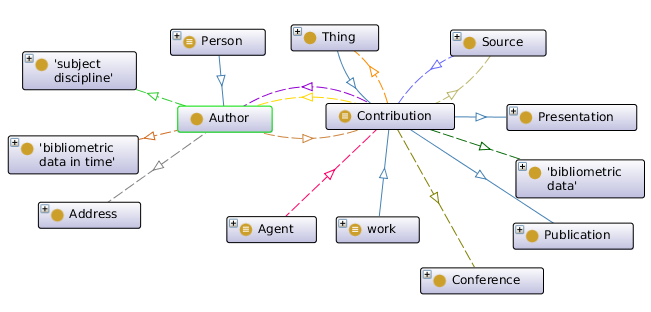
\includegraphics[width=0.9\textwidth]{./imagens/dac-mainview.png}
    \caption{Taxonomia da ontologia dac}
	\label{fig:dac}
\end{figure}

\begin{figure}[!ht]
	\centering
	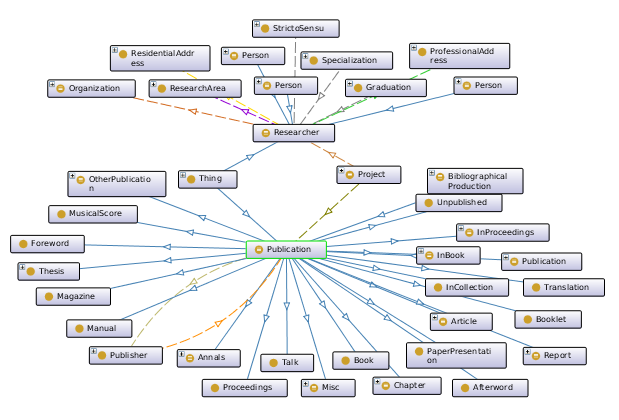
\includegraphics[width=0.9\textwidth]{./imagens/lattes-mainview.png}
    \caption{Taxonomia da ontologia lattes}
	\label{fig:lattes}
\end{figure}

Para transformar os dados para RDF foi utilizada a ferramenta OpenRefine\footnote{\url{http://openrefine.org}} com a extensão para suportar RDF. Essa ferramenta foi selecionada devido a sua facilidade para criar os templates de transformalção. Após a transformação dos dados, as ontologias e os dados foram persistidos no Virtuoso\footnote{\url{https://virtuoso.openlinksw.com}} (ver Figura \ref{fig:datasets}), que é uma ferramenta para armazenamento de triplas. O Virtuoso foi selecionado por ser uma ferramenta conhecida dos desenvolvedores.

\begin{figure}[!ht]
	\centering
	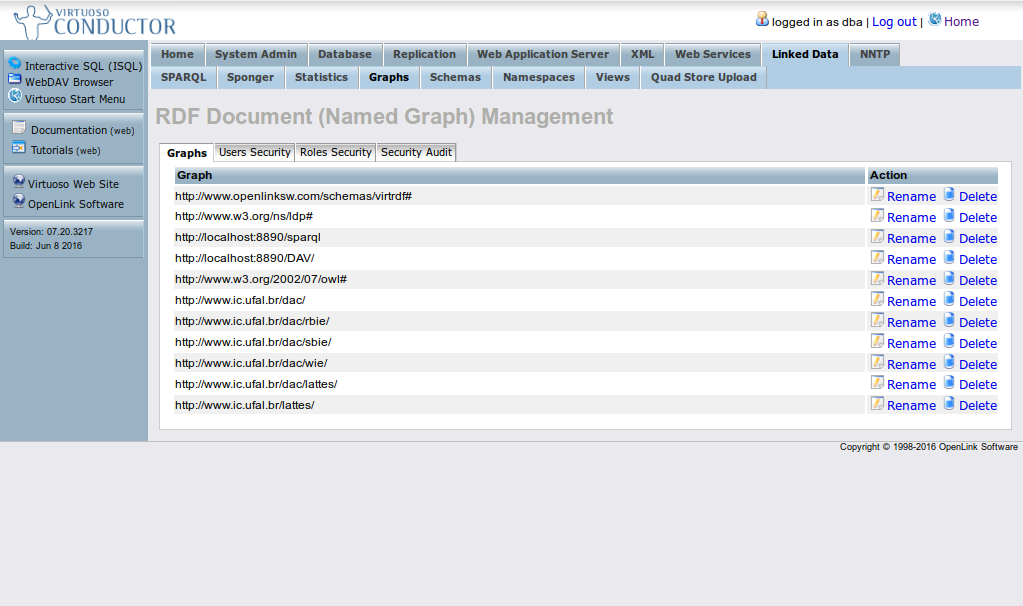
\includegraphics[width=0.9\textwidth]{./imagens/datasets.png}
    \caption{Datasets armazenados na triple store}
	\label{fig:datasets}
\end{figure}

Após a persistência dos dados, o processo de alinhamento foi executado. Vale ressaltar que os \textit{datasets} também foram alinhados com eles mesmos com o objetivo de descobrir recursos duplicados, visto que um autor pode publicar vários artigos em um mesmo evento. Os alinhamento gerados foram persistidos em novos \textit{datasets} (ver Figura \ref{fig:datasets_alingments}).

\begin{figure}[!ht]
	\centering
	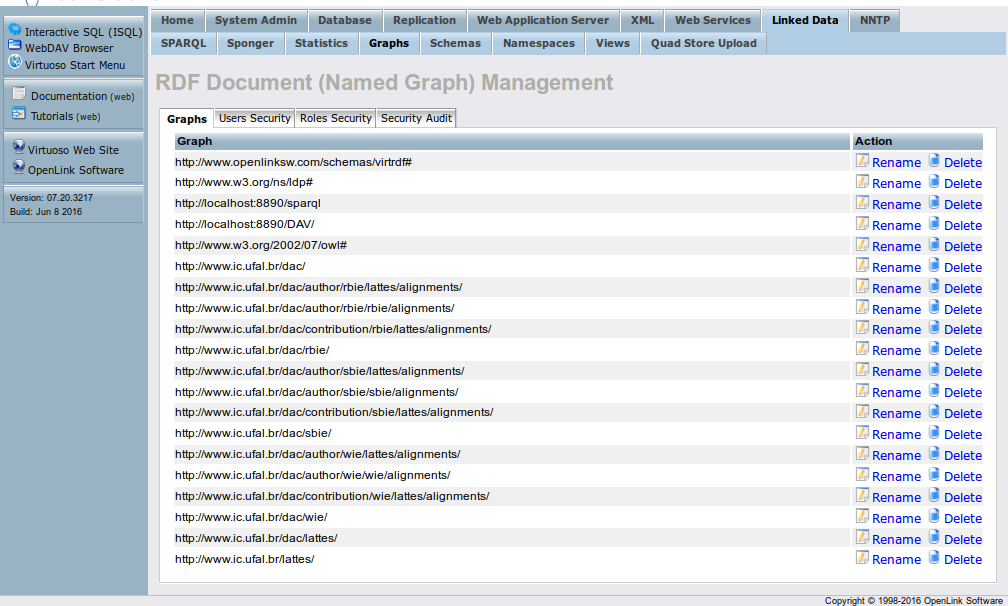
\includegraphics[width=0.9\textwidth]{./imagens/datasets-alinhamento.png}
    \caption{Datasets armazenados na triple store}
	\label{fig:datasets_alingments}
\end{figure}

Após a realização do alinhamento por parte da ferramenta, foi realizado um levantamento. A partir do levantamento foi possível gerar informações como a quantidade de recursos não repetidos nas bases, total de recursos alinhados com o perfil Lattes, bem como precisão, revocação e medida-f \cite{goutte2005probabilistic} para analisar a confiabilidade dos alinhamentos (ver Tabela \ref{tab:case_study}).

%\begin{landscape}
\begin{table}[!ht]
\centering
\caption{ Resultado dos alinhamentos com relação aos dados do Lattes}
\label{tab:case_study}
%\begin{tabular}{|p{1cm}|p{2cm}|p{2cm}|p{1cm}|p{1cm}|p{2cm}|p{2cm}|p{2cm}|}
\begin{tabular}{|c|c|c|c|}
\hline
\textbf{Dataset}	&	\textbf{RBIE}	&	\textbf{SBIE}	&	\textbf{WIE}  \\ \hline
%\textbf{Iniciais}	&	1118	&	1687	&	1952 \\ \hline
%\textbf{Alinhamentos}	&	276	&	1742	&	1637  \\ \hline
%\textbf{Recursos Alinhados}	&	1029	&	141	&	1405 \\ \hline
%\textbf{Finais}	&	806	&	1032	&	1098 \\ \hline
\textbf{Perfis com Lattes*}	&	92.03\% (1029)	&	71.54\% (1207)	&	75.20\% (1468) \\ \hline
\textbf{Perfis com Lattes**}	&	89.06\% (717)	&	70.16\% (792)	&	67.48\% (741) \\ \hline
\textbf{P | R | F}	&	0.97 | 1 | 0.98	&	0.94 | 1 | 0.97 	&	0.84 | 1 | 0.91 \\ \hline
\end{tabular}
\end{table}
* - com repetição
** - sem repetição
%\end{landscape}

Na tabela \ref{tab:case_study}, é possível notar que apesar do crescimento na quantidade de alinhamentos, a quantidade final de perfis com Lattes reduz. Isso ocorre porque a quantidade de alinhamento contabiliza a quantidade de triplas owl:sameAs, desprezando sua característica transitiva. Fato esse, que é levando em consideração quando se refere a quantidade final de recursos e a quantidade final de perfis com Lattes.

Como próximo passo, os \textit{datasets} convertidos e os \textit{datasets} gerados a partir do alinhamento foram utilizados como fonte para as consultas SPARQL. O código \ref{lst:sparql3} apresenta a consulta utilizada para contabilizar a quantidade de pesquisadores em IE. 

\begin{lstlisting}[captionpos=b, caption=Query SPARQL para recuperação de conceitos relacionados, label=lst:sparql3,
   basicstyle=\ttfamily,frame=single]
prefix dac: <http://www.ic.ufal.br/dac/>
select count(distinct ?s) count(distinct *)
from <http://www.ic.ufal.br/dac/rbie/>
from <http://www.ic.ufal.br/dac/author/rbie/rbie/alignments/>
where{
	?s a dac:Author; owl:sameAs* ?o. 
	filter not exists {
		graph<http://www.ic.ufal.br/dac/author/rbie/rbie/alignments/>{?k owl:sameAs ?s}
	}
}
\end{lstlisting}

O resultado dessa e de outras perguntas foram reunidos e uma apresentação (disponível em \url{https://goo.gl/C9nDSw}) que foi apresentada a comunidade.

